% !TEX program = xelatex

\documentclass[10pt,final]{article}
\usepackage{amsmath}
\usepackage{titlesec}
\usepackage{graphicx}
% \usepackage{sidecap} % captions on the side
\usepackage{floatrow}
\usepackage[scientific-notation=true]{siunitx} % siunits and numbers
\usepackage{caption}
\usepackage{helvet}
\renewcommand{\familydefault}{\sfdefault}
\usepackage{subcaption}
\usepackage[color=purple!40,obeyFinal]{todonotes}
\usepackage[margin=0.5in]{geometry}
\usepackage{cleveref}
\usepackage{microtype} %sexy kerning
\usepackage{color} % colors
\usepackage{ulem} % strikethrough
\usepackage{commath}
\usepackage{ifdraft}
\usepackage[	backend=biber,
		style=numeric-comp,
		sorting=none]{biblatex}
\addbibresource{ace.bib}
\floatsetup{heightadjust=object}
\date{}
\titleformat{\subsection}
  {\normalfont\fontsize{11}{17}\sffamily\bfseries\slshape}
  {\thesubsection}
  {1em}
  {}
\DeclareSIUnit\Molar{\textrm{m}}

\setcounter{secnumdepth}{4} % paragraph acts as subsubsubsection
\newcommand{\subsubsubsection}[1]{\paragraph*{#1}}
\renewcommand*{\bibfont}{\scriptsize}
% toggle for displaying instructions
\newif\ifinstr
\instrtrue

%If true, display \instr wrapped text, but only if draft mode on
\newcommand{\instr}[1]{\ifdraft{\ifinstr {\color{cyan}\emph{#1}} \fi}{}}

%pKa formatting
\newcommand{\pKa}{p$K_\mathrm{a}$\ }
\newcommand{\pH}{p$\mathrm{H}$\ }

\begin{document}
\listoftodos[Indexed list of activities pertaining to labor that will be performed in the short-term future]\newpage
\section*{\centering Specific Aims}
Among the most fundamental molecular interactions in biology are those of small molecules with their macromolecular partners.
%
Endogenous small molecules play the role of messengers in many signaling pathways of the cell, and small molecule drugs interact with proteins in signaling cascades to modulate their function.
%
Understanding their interactions is vital to understanding many biological systems, and critical to drug development efforts.
%
Despite having catalogued many of the physical driving forces behind small molecule recognition, there are enormous gaps in our knowledge preventing us from articulating a quantitative, predictive understanding of small molecule affinities and selectivities for biomolecules.

In principle, alchemical free energy calculations provide a framework for quantitatively describing all aspects of the thermodynamics of small molecule recognition. 
%
However, deficiencies in our quantitative understanding of binding create large challenges in the ability of these calculations to reproduce experimental affinities in many systems, holding back their use in probing function and aiding design.
%
\textbf{In this proposal, we address three of the most significant open challenges in the quantitative modeling of small molecule recognition by alchemical free energy calculations}.

\paragraph*{Aim 1. Establish a correct quantitative treatment of alchemical free energy calculations for binding of charged ligands.}
The predominant soluble form of many drugs and endogenous small molecules is charged.
%
Yet, retrospective studies and predictive challenges show current free energy methods make substantial errors in the treatment of binding by charged species~\cite{Rocklin2013b,Muddana2014a}.
%
A number of corrections for calculations with charged ligand species have been proposed~\cite{Reif2013a,Rocklin2013a, Lin2014a}, but (1) consensus, and (2) a good model system to test and to confirm theory are lacking.

We propose using a computationally and experimentally tractable model system---the association of small-molecule guests with high-affinity supramolecular hosts---as a way to test, validate, and refine both theory and algorithms applicable to charged ligands.
%
The experimental datasets collected here will allow us to evaluate proposed corrections to free energy calculations in order to refine theory and algorithms as necessary.
%
We will utilize isothermal titration calorimetry (ITC) experiments, which provide a “gold standard” biophysical assay for binding affinities.
%
We will additionally develop Bayesian approaches to accurately quantify measurement uncertainty and allow for model-error propagation to rectify deficiencies in current data analysis protocols.
%
\textbf{It is impossible to distinguish between experimental errors and errors in theory without accurately quantified uncertainty.
}

\paragraph*{Aim 2. Quantify the magnitude of protonation state effects on binding.}
Proteins and many small-molecule drugs contain titratable moieties that can change protonation state upon binding or sample mixtures of protonation states, often in a conformation-dependent manner.
%
While detailed biophysical studies of a few specific model systems have demonstrated that these effects can contribute several kcal/mol in binding affinity~\cite{Dullweber2001a,Aleksandrov2007a,Czodrowski2007a,Steuber2007a,Czodrowski2007b}, \textbf{the true scope and magnitude of the protonation state effects in ligand recognition in general is completely unknown.}

We will use computational techniques to conduct a survey to assess the importance of protonation state issues for a tractable but disease-relevant system---kinase catalytic domains that can be expressed in \textit{E. coli}.
%
Existing \pKa prediction tools will be benchmarked against experimental kinase inhibitor \pKa data, and then used as input for constant-\pH alchemical free energy calculations.
%
Using free energy calculations we can quantify the contribution of protonation state effects, which can be validated by performing complementary experiments.
%
We will perform ITC experiments using buffers of different ionization enthalpies that allow for deconvolution of binding and protonation states effects.

\paragraph*{Aim 3. Develop a framework for alchemical free energy calculations to describe weak association and cooperative ligand binding.}
Weak binding and association of multiple ligands are ubiquitous interactions in biological and pharmaceutically relevant systems.
%
In addition, drug discovery approaches such as fragment-based ligand design depend predominantly on a reliable method for integrating data from biophysical experiments with modeling for these situations.
%
We will extend the framework of alchemical free energy calculations  to include the potential for multiple (possibly weak) binding events using a semi-grand canonical ensemble formalism.
%

As a model system, we will use the pharmacologically relevant protein human serum albumin(HSA), known to multivalently bind many different small molecules to a variety of distinct binding sites.
%
\textbf{Most theory and frameworks focus on 1:1 interaction.}
%
We will extend deficiencies by both developing new Bayesian ITC experimental analysis techniques to select among theoretical association models,
%
as well as simulating ITC data directly from semi-grand canonical ensemble simulations.

\subsection*{} % Add some spacing

Completion of the work will provide modeling strategies for non-trivial challenges in protein-ligand association that currently have no working solution, as well as illustrate the scope of challenges that remain.

\section*{Research Strategy - Significance}
\instr{General background, significance in terms of basic science and disease relevance.}

\todo[inline,color=purple!40]{section on charged ligands}
\subsection*{Accurate treatment of alchemical free energy calculations.}
%Maybe you want to start with a section on why computer modeling or free energy calculations is important, to motivate the question of why we should care about making errors in these calculations due to incorrect protonation states?

The binding free energy of a ligand (the affinity) determines to what degree it will spontaneously associate with a protein.
%
Access to information such as free energies is of great help in the design of ligands that can selectively and tightly interact with a biomolecular target.
%
Alchemical free energy calculations are a powerful computational tool for predicting binding free energies, as they allow for efficient sampling of the relevant states of protein-ligand complexes~\cite{Shirts2007a}.
%
Unfortunately, broadly applying free energy calculations comes with several challenges that have yet to be solved~\cite{Chodera2011a,Gapsys2015a}. 

%
\textbf{Neglecting terms such as interactions with charged ligands~\cite{Rocklin2013b,Muddana2014a},
effects from changes in ligand protonation state~\cite{Dullweber2001a,Aleksandrov2007a,Czodrowski2007a,Steuber2007a,Czodrowski2007b},
and weak interactions~\cite{Gilson1997a}, has a great impact on the applicability of alchemical free energy calculations.
}%
There is need for validation  and extension available methods to allow for applying alchemical binding free energy calculations to wider ranges of systems,
thereby increasing their utility in drug discovery and development processes.


\subsubsection*{Alchemical free energy calculations need to be extended with a correct method for treating charged ligands.}
In order to apply alchemical free energy calculations to charged ligands, one needs to eliminate artifacts introduced into the calculation from various sources.
%
In a physical system, the interaction never actually disappears though the interaction between a ligand and protein is weakened to the extend that it there is no measurable correlation between the interacting molecules.
%
The elimination of a charge from a system is therefore not a physical process, and is merely an artifact of using artificial infinite systems to approximate a macroscopic system of bulk liquid.
%
Bulk liquids are approximated in simulation, either by using periodic boundary conditions, or an implicit solvent.
%
Often, to further reduce computation cost, we introduce truncated potentials and non-Coulombic electrostatics (such as PME and reaction field potentials). 
%
These unphysical treatments bring with them several electrostatic interaction terms that are added on top of the physical binding free energy.
%
The estimated binding free energy as such needs to be corrected to eliminate these effects.
%
Not correcting for these terms can severely undermine the ability of alchemical free energy calculations to reproduce experimental binding affinities~\cite{Rocklin2013b,Muddana2014a}.


\thisfloatsetup{capposition=beside,capbesideposition={center,right}}
\begin{figure}[H]
  \centering
  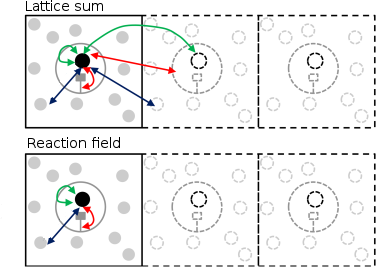
\includegraphics[width=0.4\textwidth]{figures/reif_oostenbrink.png}
    \caption{\textbf{Graphic illustration of contributions to binding free energy introduced when changing the net charge of the system.}  It is common practice to truncate Coulomb interactions beyond a certain range to reduce calculation costs and use methods such as PME or reaction fields to compensate for the loss of interaction beyond the cutoff. When there is a net charge change, this leads to errors in treatment of interaction between ligand and solvent molecules beyond cutoffs and interactions with periodic copies of the system. Figure adapted from ~\textcite{Reif2013a}.}
  \label{figure:chargecorrections}
\end{figure}

% JDC: Putting each sentence on a separate line makes it much easier to look at diffs in version control.
\subsubsection*{Unknown contributions of protonation state changes to kinase inhibitor binding affinity need to be quantified.}
The use of incorrect or inappropriate protonation states in modeling protein-ligand association can significantly degrade accuracy~\cite{Polgar2005a,Wittayanarakul2008a}.
But what if there is not a single protonation state that contributes to the binding affinity?

With the exception of a few well-studied cases~\cite{Dullweber2001a,Aleksandrov2007a,Czodrowski2007a,Steuber2007a,Czodrowski2007b}, 
the ubiquity of protonation state changes and the magnitude of their contribution to binding affinities is completely unknown. 
%
We expect there are two separate effects that may be neglected:
\begin{enumerate}
 \item A significant population of mixtures of protonation states may be present.
 \item Changes in the dominant protonation state could occur upon binding.
\end{enumerate}
%
Modeling the system with a single protonation state can in either case lead to large errors.
%
There is strong evidence that this might be the case for small molecule kinase inhibitors~\cite{Szakacs2005a,Seeliger2007a,Lin2013a}. 
%
Preliminary data (\Cref{figure:pka-kinase}) suggests that many kinase inhibitors have multiple accessible protonation states at physiological \pH.
%
Not only that, some kinase inhibitors bind with picomolar affinity to their target, corresponding to 28 $k_BT$ (16.5 $\mathrm{kcal/mole}$).
%
A 500-fold affinity loss (6 $k_BT$ , equivalent to 2.6 log unit change in the equilibrium constant) would still maintain sub-nanomolar potency.
%
Neglecting these kind of contributions would thus lead to large errors in predicted binding affinities.
%
Such large contributions could play a significant role in the selectivity of kinase inhibitors for their targets.
%
Therefore, it is essential to know whether these effects need to be incorporated if one wishes to use alchemical free energy calculations for the prediction of kinase inhibitor binding affinities.

\begin{figure}[H]
\centering
\begin{subfigure}{.4\textwidth}
  \centering
	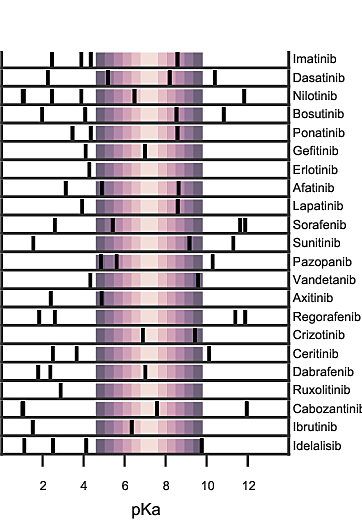
\includegraphics[width=0.95\linewidth]{figures/inhibitor-pKas.png}
	\caption{Protonation states accessible to FDA approved kinase inhibitors. Colors indicate accesibility of states at \pH 7.2 within blocks of $k_BT$ units of energy, where darker means more units of $k_BT$ away from the accesible region, up until 6 $k_BT$. Preliminary data obtained using Epik.~\cite{Shelley2007a,Greenwood2010a}}
	\label{figure:pka-kinase}
\end{subfigure}%
\hfill{}
\begin{subfigure}{.4\textwidth}
  \centering
  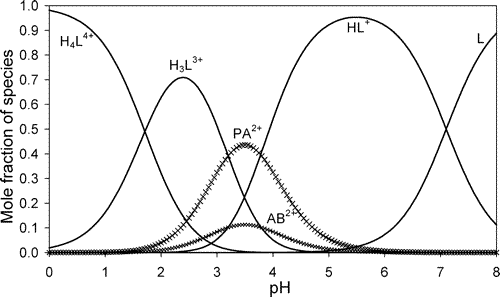
\includegraphics[width=0.95\linewidth]{figures/imatinib_curve.png}
  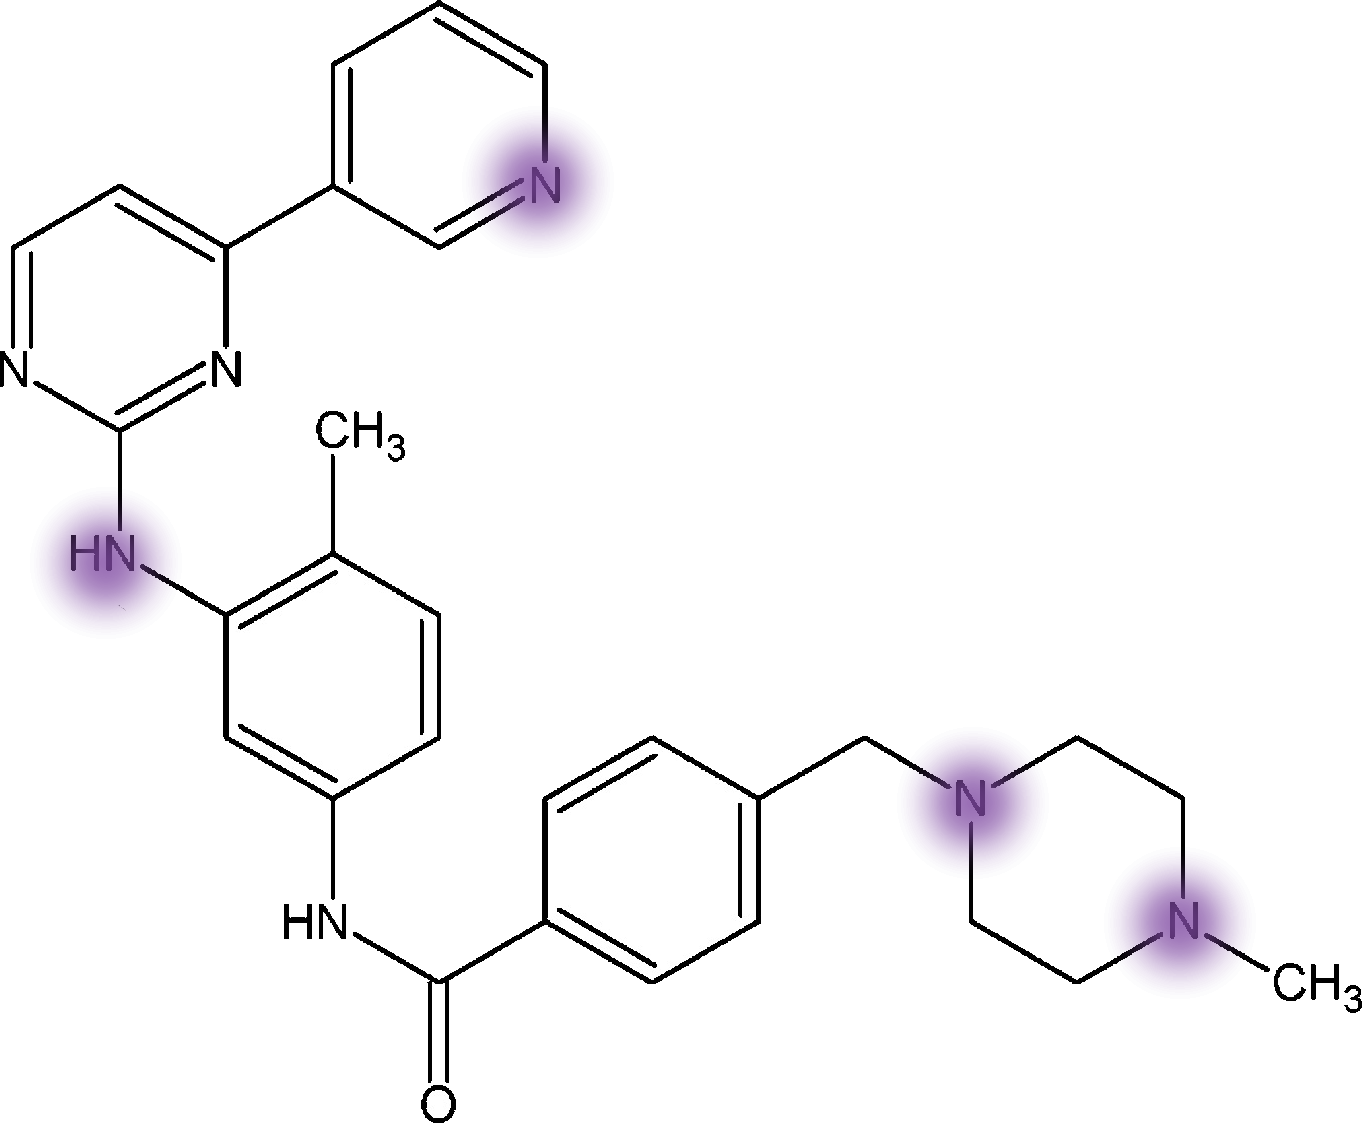
\includegraphics[width=0.95\linewidth]{figures/imatinib_groups.png}
  \caption{Top: fraction of species of imatinib (Gleevec) measured by titration and NMR~\cite{Szakacs2005a}, Bottom: The individual sites of protonation of imatinib, highlighted in purple\cite{Szakacs2005a}.}
  \label{figure:imatinib-pKa}
\end{subfigure}
\caption{}
\label{figure:kinase-pKa}
\end{figure}



% JDC: See my paragraph on this in the Significance section of the protonation state proposal.  There is also experimental evidence and multiple computational papers (Simonson papers too).
These effects have to be quantified if one's goal is not just to answer what determines the selectivity of imatinib, but also to accurately calculate its binding affinity using alchemical free energy calculations.
% JDC: You're not quite getting across the message on why this is important.  How big are the effects if you neglect this? Why is this even important?  Maybe you want to start with a section on why computer modeling or free energy calculations is important, to motivate the question of why we should care about making errors in these calculations due to incorrect protonation states?



\section*{Research Strategy - Innovation}
\instr{Explain how your proposal differs from what others have tried.}
\subsubsection*{Reliable uncertainty estimates of isothermal titration calorimetry results by using Bayesian inference.}
The ABRF-MIRG'2 study revealed the disturbing fact that the uncertainty of ITC experiments is underestimated by several orders of magnitude by conventional analysis methods~\cite{Myszka2003a}. Panel D of \Cref{figure:abrf-mirg2} indicates a statistical uncertainty of at least 10\% in the estimation of extinction coefficients between all participants of the study, which correlates linearly with errors in the concentrations of the solutions prepared by each lab. This error is propagated into the estimates of binding stoichiometry, affinity and enthalpy  (Panels A, B and C of \Cref{figure:abrf-mirg2}).

By only performing technical replicates  and no repeat experiments, the true uncertainty can not be quantified, hence no hypothesis can be supported from any single experiment~\cite{Vaux2012a}. That said, one can get an estimate of the uncertainty by performing Bayesian inference on experiments. For this reason, we propose the useage of Bayesian statistics as a means of uncertainty estimation as opposed to errors from model fit based on single or replicate experiments. Bayesian ITC can contribute to get more value out of single experiments by allowing for uncertainty quantification in concentrations of solutions. 

\thisfloatsetup{capposition=beside,
capbesideposition={center,right}}
\begin{figure}[H]
	\centering
	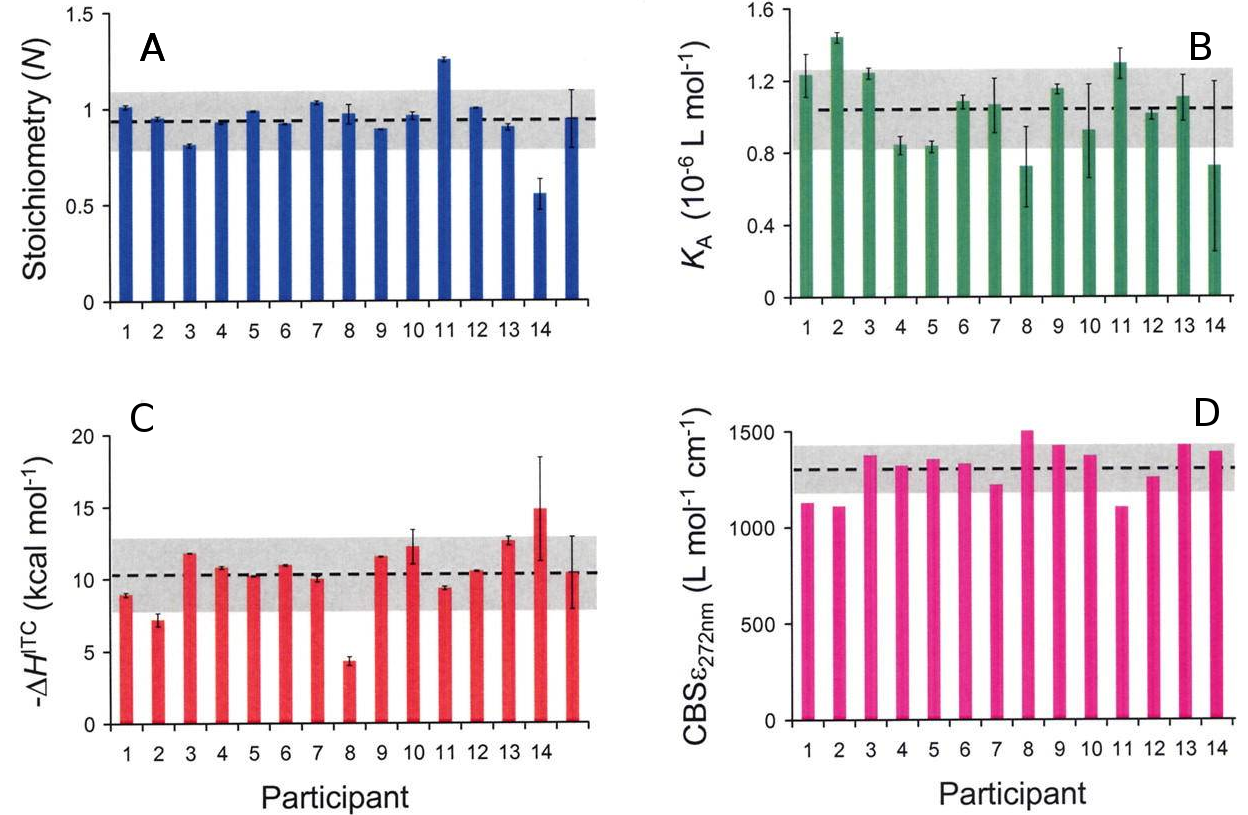
\includegraphics[width=0.49\textwidth]{figures/cbs_ca_II.PNG}
	\caption{Binding measurements from the ABRF-MIRG'2 study that considered binding of CBS to carbonic anhydrase using \textbf{ITC as performed by 14 labs shows individual error estimates that are orders of magnitude under the actual error.} A: Predicted stoichiometry of binding. B: Association constant $K_\mathrm{A}$. C: enthalpic contribution to binding. D: Measured extinction coefficient of ligand CBS, as reported by the 14 participants.~\cite{Myszka2003a}}
	\label{figure:abrf-mirg2}
	\todo[inline,color=purple!40]{need more detail here on what this data shows. can describe that same sample was distributed to 14 laboratories to measure affinity by ITC and that reported errors were orders of magnitude smaller than actual experimental variation. Also helpful to boldface first sentence of caption that succinctly summarizes figure. like ``Current ITC data analysis approaches drastically underestimate true experimental error.''}
\end{figure}

\subsubsection*{Quantifying and assessing correctness of poorly studied charge contributions to alchemical free energy calculations.}
That there is a problem describing charged ligands in alchemical free energy calculations has been pointed out multiple times in the past~\cite{Rocklin2013b,Muddana2014a}. 
%
For this reason, several possible ways of correcting this have been suggested~\cite{Reif2013a,Rocklin2013a}. A quantitative comparison is lacking, and the correctness of these methods has not been established.
%
By providing an experimental dataset with small and quantified uncertainty, we can provide a comparison of these methods that gives reasonable certainty to whether observed errors are experimental in origin, or are an error in the alchemical free energy theory. 
%
We can then not only provide a qualitative comparison on whether the models can possibly reproduce experiments, but will have a quantitative estimate of whether they produce the correct result.
%
These corrections may also prove to be necessary when performing constant-\pH calculations, where protons carrying single units of charge may come into and leave the simulation system.

\todo[inline]{How common are charged ligands? How does it affect calculations when we don't correct them?}

\subsubsection*{Computational prediction of the association of weak binders is an unsolved problem in fragment based drug discovery.}
Fragment based drug discovery (FBDD) screens a small library of fragments against a biomolecular target, where weak hits are combined to develop lead compounds.
%
The approach is frequently applied and has impacted the way the pharmaceutical industry and academia alike approach small molecule design~\cite{Hajduk2007a}.
%
The association of these fragments is hard to model computationally, because of the challenges associated with modeling weak interactions.
%
For instance, because of the absence of a strong signal that two compounds are ``bound'' to each other, it can be hard to define binding~\cite{Gilson1997a}. 


\subsubsection*{Estimating free energies of multiple ligands using semi-grand canonical ensemble free energy calculations.}
Currently, there is no available framework to perform alchemical free energy calculations that allowing for an arbitrary amount ligands to associate with a single protein.
%
We propose to extend the available toolset of the computational chemist with semi-grand canonical ensemble methods that enable the calculation of binding affinities of multiple ligands to multiple sites.
%
As opposed to simulating a single ligand at multiple sites, this way we can correctly take into account cooperativity in binding when multiple ligands associate with a single protein.

\subsubsection*{Providing an estimate of the prevalence and magnitude of protonation state event contributions to kinase inhibitor binding}
\todo[inline,color=purple!40]{write this section, inspiration from the kinase proposal}


\section*{Research Strategy - Approach}
\instr{Approach: More specific background information. Describe in detail the experimental design and research methods to be used. Technical hurdles to be overcome should be mentioned. Alternative approaches should be given for experiments that may not be feasible. Discussion of expected or possible results and their interpretation. Best format for each specific aim: a) rationale, b) methods, c) expected results, d) alternatives. Theory aims should follow a similar structure where possible.}


\subsection*{Aim 1. Establish a correct quantitative treatment of alchemical free energy calculations for binding of charged ligands}
\subsubsection*{Rationale}
The soluble form of many drugs and endogenous small molecules is charged. Yet, retrospective studies and predictive challenges show current free energy methodology makes substantial errors in the treatment of binding by charged species~\cite{Rocklin2013b,Muddana2014a}.
%
For explicit solvent simulations using particle mesh Ewald ---the gold standard approach to simulating solvated biomolecular systems--- a number of details of the calculation impact macroscopic observables when the total charge of the system or the overall charge density changes by removal of a charged ligand.
%
A number of approaches for explicitly solvated PME free energy calculations with charged species have been proposed, but (1) consensus, and (2) a good model system to test and to confirm theory are lacking~\cite{Reif2013a, Rocklin2013a, Lin2014a}.

We propose using the association of small-molecule guests with high-affinity supramolecular hosts as a way to test, validate, and refine both theory and algorithms applicable to charged ligands.
%
We will use cucurbit[7]uril~\cite{Lagona2005a} (CB7) as a host, which is known to bind a series of cations within a range of affinities spanning several orders of magnitude~\cite{Cao2013a} (see \Cref{figure:host-guest}).
%
In order to provide an experimental dataset with accurately quantified uncertainty, we will perform isothermal titration calorimetry (ITC) experiments of various guests binding to CB7.
%
We will then perform alchemical free energy calculations to evaluate the available approaches in an attempt to support or refute them.

%
ITC experiments will benefit from the high solubility of CB7.
%
CB7 is more soluble than a lot of proteins, \SIrange[scientific-notation=false]{20}{30}{millimolar}~\cite{Lagona2005a} in water versus \textless \SI{1.0}{millimolar} for a small ``soluble'' protein such as RNAase Sa~\cite{Pace2004a}.
%
This will allow us to reach higher concentrations, which will make for more tractable experiments.

The small system size provides an advantage for molecular dynamics simulation, since the limited degrees of freedom will make sampling more efficient and reduces computational cost.
%
Unlike biomolecules, CB7 does not undergo large-scale conformational changes and has small correlation times.

\begin{figure}[H]
\centering
\begin{subfigure}{.5\textwidth}
  \centering
  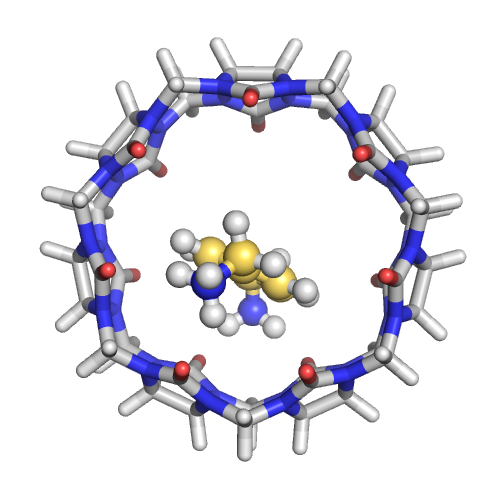
\includegraphics[width=.4\linewidth]{figures/guest11_top.png}
  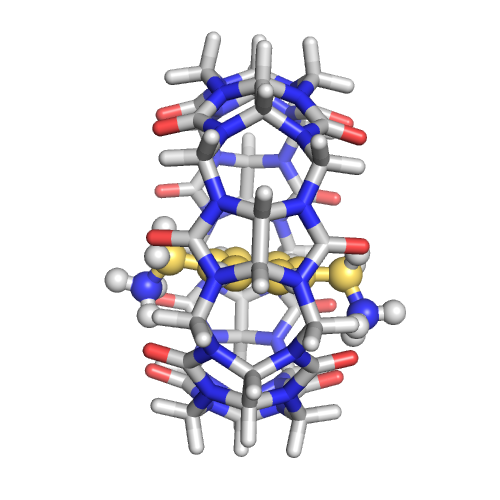
\includegraphics[width=.4\linewidth]{figures/guest11_side.png}
  \caption{Guest 11~\cite{Cao2013a} bound to the central cavity of CB7.}
  \label{fig:sub1}
\end{subfigure}%
\begin{subfigure}{.5\textwidth}
  \centering
  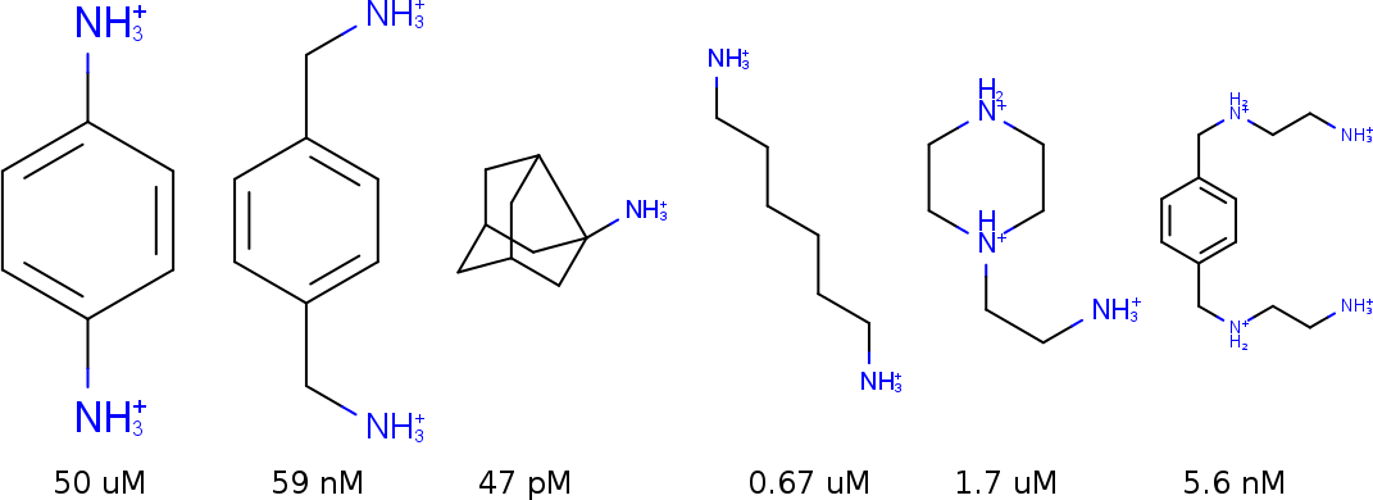
\includegraphics[width=0.95\linewidth]{figures/Kd_guest.png}  
  % JDC: All of the guests are scaled in weird ways making benzene rings different sizes.  Would be great to fix this at some later point, but not essential now.
  \caption{A selection of guests and their $K_d$ values from \textcite{Cao2013a}.}
  \label{fig:sub2}
\end{subfigure}
\caption{\textbf{Cucurbit[7]uril (CB7) bound to several cationic guests from \textcite{Cao2013a}}. Different guests bind to the central cavity of CB7, though their affinity is determined by their geometry and size. Their affinities are in a range similar to many protein-ligand complexes, though the complexes are small, with few degrees of freedom, making them excellent candidates for our study. Figure prepared using Glide docking~\cite{Halgren2004a,Friesner2004a,Friesner2006a,Schroedinger2014a} into crystal structure pdb:QQ7~\cite{Feng2004a}.}
\label{figure:host-guest}
\end{figure}

ITC has been shown to lead to serious underestimation of measurement error due to failure to propagate errors in the concentration of reactants\cite{Myszka2003a,Tellinghuisen2011a}. To provide an accurate assessment of error from single experiments, we will develop a novel analysis method using Bayesian inference.
%
The framework of Bayesian inference allows for the propagation of errors throughout the experimental procedure, allowing us to accurately quantify the experimental uncertainty, thereby enabling us to clearly refute or support the various approaches to dealing with charged ligands.

We will consider the approaches of \textcite{Reif2013a}, \textcite{Rocklin2013a}, and \textcite{Lin2014a} for eliminating the contribution of net charge.  Each scheme mostly agrees on the source of error, but has a different way of solving the problem, as described in subaim 1.2. 

We will also consider the elimination of neutral salt pairs, in lieu of corrections, to evaluate the necessity of these complex schemes.


\subsubsection*{Subaim 1.1: Develop an accurate approach to quantifying experimental uncertainty in ITC using Bayesian inference.}
To test and confirm theoretical models, an accurate quantitative estimate is needed of the experimental error of the experiments that are used to validate.
%
We will develop Bayesian approaches to accurately quantify measurement uncertainty and allow for model-error propagation. 
Errors in the concentration of prepared solutions are a major source of uncertainty in ITC data. Not taking these into account can lead to orders of magnitude underestimation of the uncertainty of the experiments~\cite{Myszka2003a,Tellinghuisen2011a}.
One way to take this into account is by doing repeat experiments in which all solutions are prepared anew for each replicate, instead of technical replicates~\cite{Vaux2012a}. This however is time and material consuming, and therefore not a popular option among most scientists. 

In a Bayesian approach, we can assign prior distributions to the true concentrations of both species, allowing the uncertainty in these concentrations (tracked during solution preparation via standard propagation of error) to be used as input.
Using \textit{Markov Chain Monte Carlo} (MCMC)~\cite{Metropolis1953a,Hastings1970a}, we can then sample from a joint posterior probability distribution of all thermodynamic parameters to estimate the actual concentration, using\textit{Bayes' rule} 
%
\begin{align}
	\mathcal{P}\left(\theta | \mathcal{D} \right) \propto  \mathcal{P}(\mathcal{D} | \theta) \mathcal{P}\left(\theta\right) \quad;\quad \theta   =  \left\{ \Delta G_\mathrm{bind}, \Delta H_\mathrm{bind}, \Delta H_0, [\mathrm{X_{syr}}], [\mathrm{M_{cell}}], \sigma \right\}
\end{align}
%
where $\mathcal{P}(\mathcal{D}|\theta)$ is the likelihood of the data $\mathcal{D}$ (i.e., injections heats $q_n^\mathrm{obs}$), given the individual thermodynamic parameters $\theta$, and $\mathcal{P}(\theta)$ is a prior distribution of the set of independent thermodynamical parameters. Our posterior model contains parameters such as the binding affinity ($\Delta G_\mathrm{bind}$), the enthalpy of binding ($\Delta H_\mathrm{bind}$), an offset to incorporate mechanical and dilution effects ($\Delta H_0$),  the true reagent concentrations in the syringe ($[\mathrm{X_{syr}}]$), and in the sample cell ($[\mathrm{M_{cell}}]$), and $\sigma$, the square root of the variance of our measurements.

The simplest likelihood model of an ITC experiment consist of a series of $n$ injections, resulting in injection observed heats $q_n^\mathrm{obs}$,
%
\begin{align}
	q_n^\mathrm{obs} \sim \mathcal{N}(q_n^\mathrm{true}, \sigma^2) \quad ,
\end{align}
%
which are drawn from a normal distribution $\mathcal{N}$ with a variance of $\sigma^2$ and with the true injection heats $q_n^\mathrm{true}$ as the underlying mean. As stated by the central limit theorem (CLT), the sum of the individual power measurements, integrated to give the heat of single injections, will be normally distributed.

The methodology will allow incorporation of multiple experiments, such as calibrations, to accurately separate out heat effects due to e.g. dilution of the chemicals used or mechanical effects of the injections.

We will collect ITC data for the series of guests used by \textcite{Cao2013a} binding to CB7. Experiments will be performed using an Auto iTC-200 instrument, available at the Rockefeller University High-Throughput and Spectroscopy Resource Center (HTSRC). The experimental setup will be designed using a python library  developed in house for the design of ITC experiments, and the setup will be carried out on our in house laboratory automation system using procedures generated by the library.

\subsubsubsection{Subaim 1.2: Perform a quantitative comparison of suggested correction models to experiments to establish a correct treatment of charged ligands in alchemical free energy calculations.}
We will compare several methods that correct for changes in net charge of the system in alchemical free energy calculations~\cite{Reif2013a,Rocklin2013a, Lin2014a} in order to estimate which methods can provide quantitatively correct estimates of the binding affinity.
%
To do so, we will perform alchemical binding free energy calculations on the series of guests-CB7 complexes for which binding affinities were measured as part of subaim 1.1 and compare the methods to the experimental results.

We will consider a total of four schemes that account for charged ligand binding.
%
The approach of \textcite{Reif2013a} uses a thermodynamic cycle to define a raw charging contribution to binding free energy, and tries to deconvolute the various contributions so that they can be subtracted from the total binding free energy.
%
\textcite{Rocklin2013a} suggests a numerical, as well as an analytical scheme to calculate contributions, both using Poisson-Boltzmann (PB) calculations on the protein-ligand system.
%
Then, there is the approach of \textcite{Lin2014a}, who use potential of mean force (PMF) calculations in a single simulation system with a macromolecule and ligand unbound, separating them by a large distance in explicit solvent.
%
We will also test an additional model that does not apply corrections, in which a neutral ligand:counterion pair is alchemically eliminated. 


%
We will first consider whether all methods agree with each other, and the extent of the difference between their estimates.
%
Discrepancies between the results could indicate that some of the approaches are quantitatively incorrect.
%
If the various approaches agree, we can compare them in terms of efficiency.
%
Next, we will compare each of the approaches to the experimental data, to see whether any of them produce a quantitatively correct result.
%
The accurately quantified uncertainty of our experimental data will provide us with a means to refute or buttress the proposed correction schemes.




\subsubsection*{Expected results}
The ITC experiments performed on the CB7-guest complexes will be analyzed using our Bayesian ITC analysis method.
%
This will provide us with estimates of their binding affinity with accurately quantified uncertainty. 
%
Then, we will perform alchemical binding free energy calculations, in an attempt to reproduce the experimental data.
%
We will evaluate whether each of the individual schemes produces the same answer and will estimate the difference between their estimates. 
%
Next, we can compare the result obtained by each scheme to the experimental results. If their estimate falls within the range of the experimental estimate, then it supports the suggested approach.
%
Each of the methods carries an increased computational cost with them, compared to not applying corrections.
%
By applying them on the same system, we can also get an estimate on how efficient they are in costs versus improved accuracy.

We will then be able to recommend a methodology to use when calculating the free energy of binding for charged species, enabling reliable simulations that are impossible to perform otherwise.
% JDC: Maybe try a different approach here: How will you actually analyze the data?  First, you'll see which, if any, of the computational techniques agree with each other, and if not, by how much they differ.  Then, you will see if any of the methods agree with experiment.  If so, this buttresses these approaches; if none of the methods agree, then you can investigate other issues (none of the methods may be correct or there may be forcefield issues).  Finally, you can also compare the efficiencies of these different computational techniques.

\subsubsection*{Pitfalls and alternatives}

\todo[inline,color=purple!40]{modulate strength of interactions by modulating salt concentration}
It is possible that all methods produce comparable results, in which case we can perform a comparison of efficiencies to determine which method is best.
%
Another potential outcome is that none of the models are able to reproduce the experimental results.
%
This could indicate problems with the force field used to simulate the systems.
%
We can use a variety of different force fields to estimate errors that are due to the force field.
%
For instance, we could compare the GAFF\cite{Wang2004a}, GAAMP\cite{Huang2013a}, and OPLS\cite{Schroedinger2014b} force field models to get an estimate of the force field error. 

To further estimate force field error, we could perform the same experiments and alchemical free energy calculations using a neutral guest. 
%
This would leave out the contribution due to a net charge change, so that the accuracy of the force field can be assessed.


\subsection*{Aim 2. Quantify the magnitude of protonation state effects on binding}
\subsubsection*{Rationale}
Proteins and many small-molecule drugs contain titratable moieties that can change protonation state upon binding or sample mixtures of protonation states, often in a conformation-dependent manner.
%
While detailed biophysical studies of a few specific model systems have demonstrated that these effects can contribute several kcal/mol in binding affinity~\cite{Dullweber2001a,Aleksandrov2007a,Czodrowski2007a,Steuber2007a,Czodrowski2007b},
the ubiquity and magnitude of protonation state effects in ligand recognition in general is unknown.
%
The usual approach in modeling ignores these problems and assumes a single protonation state for an entire system.
%
By doing so, contributions of unknown magnitude are ignored.
%
Our aim is to develop a framework that can combine \pKa predictions of small molecules with alchemical binding free energy calculations in a constant-\pH setting.
%
We will then use this framework to quantify the effect of protonation state effects on the binding of kinase inhibitors.


We will first validate whether the existing \pKa methods can provide useful intrinsic \pKa s of solvated ligands, before assessing their accuracy in the use for simulating complexes.
%
We will use experimental \pKa data, obtained for a series of kinase inhibitors to benchmark the tools.
%
This will then be plugged into a titration framework called MCCE~\cite{Song2009a}, which can derive adapted \pKa values for small molecule-protein  complexes.
%
We will use available kinase-inhibitor complexes from the protein databank (PDB)~\cite{Berman2000a}, using the small molecule \pKa predictions as input.
%
Then, we will perform constant-\pH free energy calculation, feeding in the input from complex \pKa value estimates.
%
The free energy calculations will be validated by performing complimentary ITC experiments.
%
By performing multiple ITC experiments in buffers with varying ionization enthalpy, we can determine the thermodynamic contribution of protonation state effects on the total binding free energy~\cite{Baker1996a,Neeb2014a}.
%
This will allow us to validate the free energy calculations, and can provide validation on whether protonation state effects have a large contribution on the binding affinity.
%
We can then use our alchemical free energy calculation framework to predict the magnitude of protonation state effects in other systems, for which experiments have not been performed.

\todo[inline,color=purple!40]{short explanation constant-\pH simulations}

% \subsubsection*{Methods}
\subsubsection*{Subaim 2.1: Survey the utility of available small molecule \pKa predictions for use in constant-\pH alchemical free energy calculations.}
Our aim is to quantify the contribution of protonation state changes to binding interactions.
%
We will focus on a smaller subset of interactions in a tractable system, the interactions of small molecule inhibitors of kinase domains.
%
Preliminary results suggest that several kinase inhibitors have access to multiple states  at physiological \pH.
%
For instance, the intracellular \pH of most tumors is around 7.2~\cite{Griffiths1991a,Stubbs2000a}.
%
Preliminary data in \Cref{figure:pka-kinase} indicates that a number of FDA approved kinase inhibitors have \pKa values close to the physiological \pH, including imatinib~\cite{Szakacs2005a}.

In order to use a computational framework such as constant-\pH simulations, we need to provide small molecule \pKa data.
%
These calculations can benefit greatly from input by a reliable computational \pKa prediction tool, since this could directly be connected into the framework.
%
We will benchmark existing \pKa prediction tools using \pKa data obtained for a series of kinase inhibitors using a Sirius T3 instrument.
%
The Sirius T3 instrument provides a gold standard for giving macroscopic \pKa{}s using a combination of electrochemical and UV-metric titrations.)

This will provide a means to select a tool that can adequately predict \pKa values for kinase inhibitors with similar chemical components.




Among the small molecule \pKa prediction tools considered will be \textbf{MoKa}~\cite{Milletti2007a}, \textbf{Jaguar}~\cite{Bochevarov2013a}, and \textbf{Epik}~\cite{Shelley2007a,Greenwood2010a}.
%
MoKa generates \pKa{}s based on atomistic descriptors, defined by the surrounding atoms.
%
The descriptors are based on molecular interaction fields calculated using GRID~\cite{Goodford1985a} for a library of 3D fragments, but can succesfully be applied on 2D structures.
%
Schrodinger's Jaguar provides means of estimating \pKa values using quantum mechanical methods.
%
Epik uses Hammett Taft linear free energy approaches~\cite{Perrin1981a} for predicting \pKa values .
%
To accurately incorporate \pKa effects into our simulations, we also need to consider that the \pKa of protein residues may change on binding of a ligand.
%
We will survery small molecule-kinase interactions using MCCE~\cite{Song2009a}, which will be extended to incorporate small molecules in its calculations.
%
We will make a selection of crystal structures from the protein data bank (PDB)~\cite{Berman2000a} of kinases with inhibitors bound.
%
We can then selecting for systems that show potential mixtures of protonation states at physiological \pH values as indicated by their multiconformer \pKa prediction to use in constant-\pH simulation as part of our aim. 


\subsubsection*{Subaim 2.2: Estimate the effect of protonation states on binding affinity through experiment and computation.}
The obtained data from the \pKa survey will allow us to set up alchemical free energy calculations that employ semi-grand canonical contant-\pH methods.~\cite{Mongan2004a,Stern2007a,Nilmeier2011a}
\todo[inline,color=purple!40]{(Benoit Roux has just submitted a paper on this for explicit solvent too.)}

The calculations will be performed using OpenMM~\cite{Eastman2013a} and Yank~\cite{Chodera2015a}.
%
We will also perform simulations that do not apply the constant-\pH methods. This will allow us to estimate the effect of protonation state changes on the binding affinity.

We will validate the results of the free energy calculations by performing complementary experiments on kinase catalytic domains that can be expressed in E. coli using ITC experiments.
%
The change of protonation states can be observed in ITC by performing replicate experiments using buffers of different ionization energies~\cite{Baker1996a,Neeb2014a}.

This will lead to an enthalpic contribution/penalty to the binding affinity.
%
We will systematically explore the effects of fixed and dynamic protonation states on kinase, inhibitor, and kinase:inhibitor complexes to determine the impact of assuming protonation states are fixed or dynamic, and to dissect the effect in terms of protein-dominated, ligand-dominated, or coupled protein-ligand effects.
%
We will quantify the impact on errors in binding affinity.

\subsubsection*{Expected results}
The performance of constant-\pH alchemical binding free energy calculations will allow us to asses the prevalence and magnitude of the effect of protonation states on the binding of kinase inhibitors.
%
This knowledge can be used to determine whether these effects play a significant role in the selectivity of kinase inhibitors for their targets.
%
We hope to identify whether protonation state effects could have order of magnitude impacts on the binding affinity of small molecule inhibitors of kinases.
%
In the case that changes in protonation state make a significant contribution, we will now have the tools to include this in our modeling.
%
If the contribution appears to make no significant difference, we will have ruled out the need to use more expensive theoretical methods and more experimental resources.


\subsubsection*{Pitfalls and alternatives}
In the case that our computational estimates of the protonation state contributions differ from our experimental estimates, this could implicate other effects have not been incorporated into our simulation. 
%
For instance, the conformational states of the protein considered for our free energy calculations might need to be expanded.
%
We could use techniques such as Markov state models (MSM)~\cite{Prinz2011a} to determine the important metastable states of kinase systems and use this knowledge to enhance our free energy calculations.
\subsection*{Aim 3. Develop a framework for alchemical free energy calculations to describe weak association and cooperative ligand binding.}
\subsubsection*{Rationale}
Weak binding and association of multiple ligands are ubiquitous interactions in biological and pharmaceutically relevant systems.
%
In addition, drug discovery approaches such as fragment-based ligand design depend predominantly on a reliable method for integrating data from biophysical experiments with modeling for these situations.
%
When performing binding experiments, the stoichiometry is unknown a priori.
%
By using an alchemical free energy calculation framework, we can calculate the free energy of the different occupation states of a protein-multiligand complex (0, 1, $\dots$, $N_\mathrm{max}$ ligands).
%
This information can be used to predict the concentration of the various complexes in solution.
%
As part of this aim, we will develop the tools to model the association of multiple ligands using alchemical free energy calculations.
%
Additionally, we will extend our Bayesian ITC analysis framework with the ability to infer the number of independent binding sites, and complex concentrations.
%
That way, we can establish a quantitative connection between the alchemical free energy calculations, and ITC experiments of multiple association.
%
We will be able to simulate ITC experiments directly from the parameters obtained from our alchemical free energy calculations.

As a model system, we will use the pharmacologically relevant protein human serum albumin (HSA).
%
It is a protein with multiple binding sites that bind a wide variety of ligands~\cite{He1992a,Kragh-Hansen2002a,Sulkowska2002a}.
%
Its binding sites are asymmetric~\cite{He1992a, Curry1998a} and one expects there to be difference in binding affinity of a ligand for each site~\cite{Sudlow1976a} (see also \Cref{figure:albumin}))

\thisfloatsetup{capposition=beside,capbesideposition={center,right}}
\begin{figure}[H]
	\centering	
	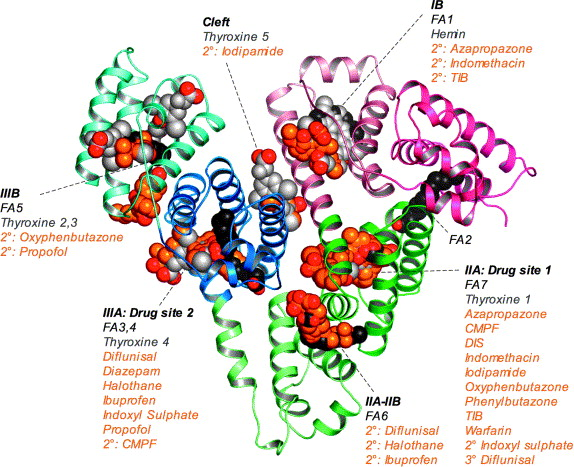
\includegraphics[width=0.49\textwidth]{figures/hsa_fig7_ghuman2005.jpg}
	\caption{\textbf{Summary of the ligand-binding capability of Human serum albumin structural studies to date.} Ligands are depicted in space-filling representation; oxygen atoms are coloured red; all other atoms in fatty acids (myristic acid), other endogenous ligands (hemin, thyroxin) and drugs are coloured dark-grey, light grey and orange, respectively. Because of the many small molecule interactions of HSA, it is expected to be of great importance to the bioavailability of small molecules~\cite{Metcalfe2010a}. It is known to bind several drugs~\cite{SJOeHOLM1979a,Bannwarth1996a,Sulkowska2002a,Ghuman2005a,Perez2007a}, as well as dietary supplements~\cite{Pal2013a}. It is also essential for the bioavailability of endogenous small molecules such as hormones~\cite{Pardridge1986a}, and toxins such as cardiac glycosides~\cite{Smith1985a}. From Figure 7 of~\cite{Ghuman2005a}.
}
	\label{figure:albumin}
	\todo[inline,color=purple!40]{show small molecules we will use}
\end{figure} 


% \subsubsection*{Methods}

\subsubsection*{Subaim 3.1: Extend semi-grand canonical ensemble alchemical free energy calculation tools.}
We wish to estimate the binding affinity of multiple ligands, associating with a single protein.
%
Alchemical free energy calculations are frequently applied to calculate the binding affinity of single ligands to a protein~\cite{Shirts2007a}. 
%
Currently, a framework to perform alchemical simulations with multiple ligands does not exist.
%
Therefore we will extend the framework of alchemical free energy calculations to include the potential for multiple (possibly weak) binding events using a semi-grand canonical ensemble formalism. 
%
In the semi-grand canonical ensemble ($\mu N_R PT)$, the number of ligand molecules is allowed to vary between 0 and $N_{max}$ , and the number of receptor molecules $N_R$ is fixed.
%
The pressure, $P$, and temperature, $T$, are also fixed. The free energy of observing $n$ ligand molecules is,
\begin{align}
 g_n = \ln \int \dif x_1 \dif x_n \dif x_R \, e^{-u_n(x_1,\dots,x_n)} \quad,
\end{align}
where  $u_n(x_1,\ldots,x_n,x_R) \equiv \beta U_n(x_1,\ldots,x_n,x_R)$ is the \emph{reduced} potential energy, based on the coordinates of $n$ ligand molecules and the receptor.

\begin{align}
 Q = 1 + K_1x + K_1K_2x^2 \dots \left(\prod\limits_{i=1}^{n} K_i\right) x^n = 1 + \sum\limits_{l=1}^n \left(\prod\limits_{i=1}^{l} K_l\right)x^l
\end{align}


\thisfloatsetup{capposition=beside,capbesideposition={center,right}}
\begin{figure}[H]
  \centering
  \fbox{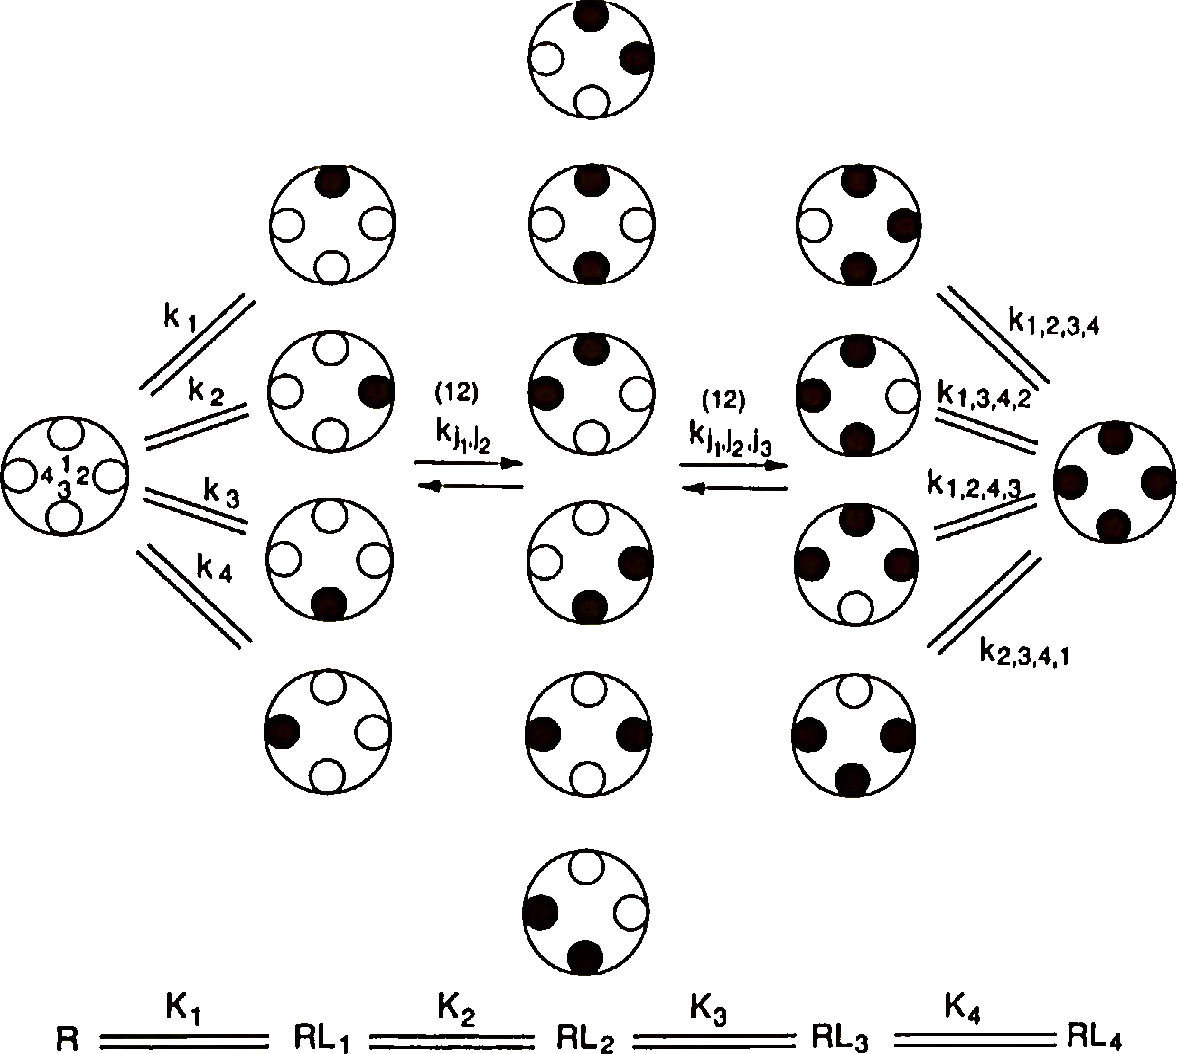
\includegraphics[width=0.4\textwidth]{figures/binding_sites.png}}
  \caption{\textbf{In the semi-grand canonical ensemble, we consider the association of 0 up to $N_\mathrm{max}$ ligands to a protein. }By using alchemical perturbations, they can be inserted without pushing the system away from equilibrium. We can calculate the free energy of associating additional ligands to the protein by using binding polynomials of the stoichiometric binding constants $K_i$. Figure adapted from \textcite{Klotz1997a}. }
  \label{figure:semigrand}
\end{figure}

\todo[inline,color=purple!40]{deficiencies in FBLD theory or in general? what are the deficiencies?}
\todo[inline,color=purple!40]{explain semi-grand canonical}

\begin{align}
K_{n+1} = \frac{[RL_{n+1}]}{[RL_n][L]} = e^{-(g_{n+1}-g_n)}
\label{eq:K_eq}
\end{align}


\todo[inline,color=purple!40]{This isn't really the main idea here.  The key idea is that we need to compute the free energy of having 0, 1, 2, 3... ligands bound to the protein for some sort of standard state volume. Then, for a given ligand concentration, we can compute the probability that a given macromolecule will have 0, 1, 2, 3... ligands bound.  We can even go further and say something about cooperativities between sites, etc.)}

Alchemical methods will allow us to insert new copies of ligands into our simulation without driving the system far away from equilibrium. 

\subsubsection*{Subaim 3.2: Validate computational predictions by applying Bayesian model selection on ITC  experiments of HSA and a series of NSAIDS.}
To provide validation of our computational results, we will perform ITC experiments on HSA.
%
Binding stoichiometry is not known a priori, yet if we want to deconvolute characteristics such as binding affinities for different sites, we need to model multiple binding sites with multiple affinities.
%
\todo[inline,color=purple!40]{stoichiometry is too primitive to describe multiple binding sites with varying affinity}
%
Using the predicted affinities and stoichiometry from alchemical free energy calculations, we can design ITC experiments that can provide maximal information on the actual associations. 
%

To analyze the experiments, we will have to develop new methodology to fit within our Bayesian ITC framework.
%
Origin, a conventional ITC analysis software package uses cooperativity parameters $n_i$ to describe multiple binding sites~\cite{MicroCal2004a} up to a maximum of two.
%
SEDPHAT additionally uses terms describing ``incompetent fractions'' of experimental components~\cite{Houtman2007a,Zhao2015b} and can deal with up to 3 sites.
%
We will extend our Bayesian analysis tools with the capacity to select between possible association models without limiting the number of distringuishable sites or binding stoichiometry.
%
At the same time, by applying correlated uncertainty estimates in the concentrations, it will be able to distinguish errors in the concentrations of the prepared solutions from changes in stoichiometry, unlike the simple Origin models. 

\subsubsection*{Expected results}
Alchemical free energy calculations can suggest the number of predicted interaction sites, as well as provide estimates for the affinity of each individual site.
This allows us to study the predicted interactions at an atomistic scale, as well as design experiments at concentrations that will provide the most detailed information, for ITC experiments that can observe multiple drugs binding to HSA at the same time, or binding to multiple sites.

\todo[inline,color=purple!40]{expected for overall aim?}

Our Bayesian ITC analysis methodology will then enable us to predict binding affinities to HSA with its multiple binding sites. We will be able to deconvolute the heat effects of multiple species, as well as multiple binding sites.

\subsubsection*{Pitfalls and alternatives}
Binding sites with multiple affinities might be hard to measure accurately with ITC if the affinities are very different. We can perform dynamic range experiments which search multiple ranges of concentration and detect binding sites. Then, using Bayesian experimental design, we can perform adaptive experiments that will yield new information that can describe all the features detected.

\todo[inline,color=purple!40]{competition experiments could be helpful, push out weak binder with strong binder?}

\section*{Conclusion}
The aims of this proposal contribute to the limited set of tools available to deal with protein-ligand interactions in special, but not rare, cases where conventional tools provide no theoretical framework. Using Bayesian methodology will provide reliable uncertainty estimates on experimental data, which in turn will enable the distinction between theoretical model errors and experimental errors.

% refs
\setlength{\emergencystretch}{1em}
\printbibliography

\end{document}

